\chapter[Appendice]{Appendice}

\begin{figure}[htpb]
	\centering
	\subfigure[]{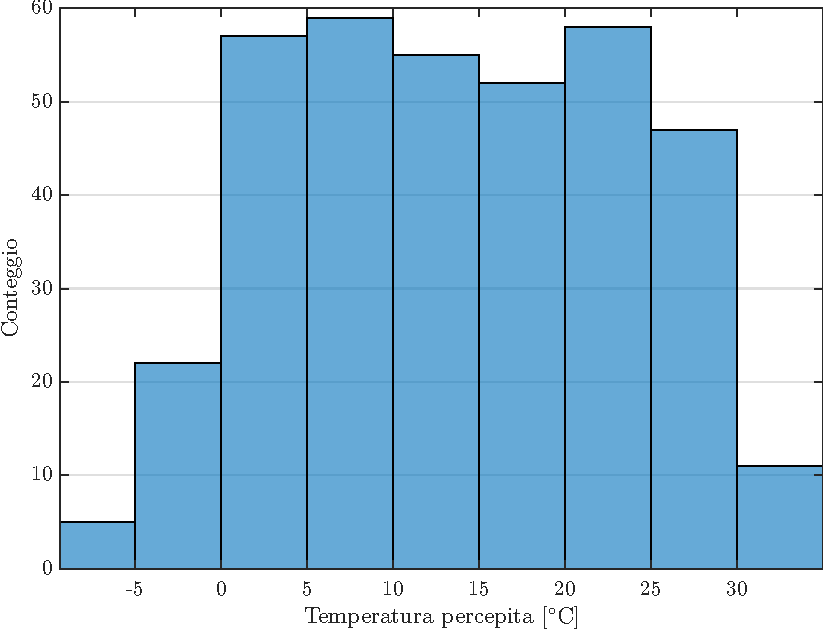
\includegraphics[height=133px]{Immagini/4. Caso di studio/Istogrammi/Istogramma, temperatura percepita}\label{istogramma_temperatura}}\quad
	\subfigure[]{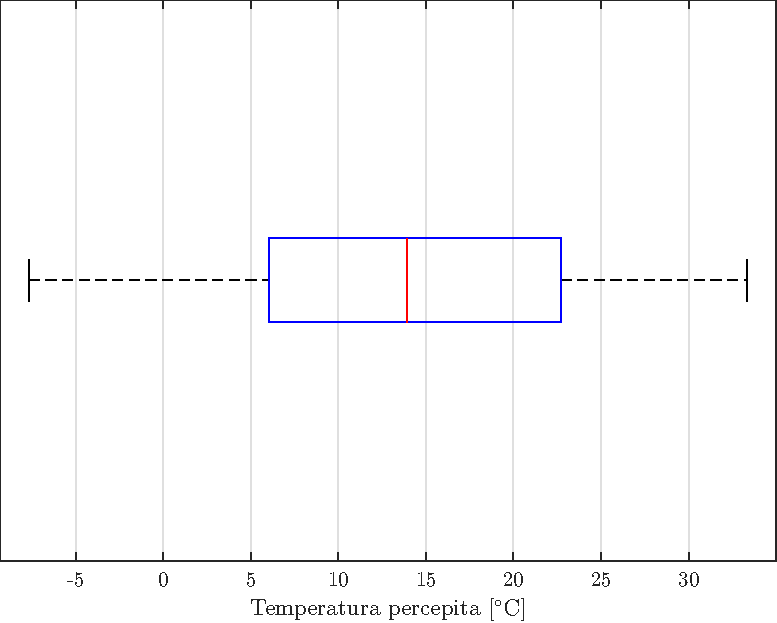
\includegraphics[height=133px]{Immagini/4. Caso di studio/Box-plot/Box-plot, temperatura percepita}\label{boxplot_temperatura}}\quad
	\subfigure[]{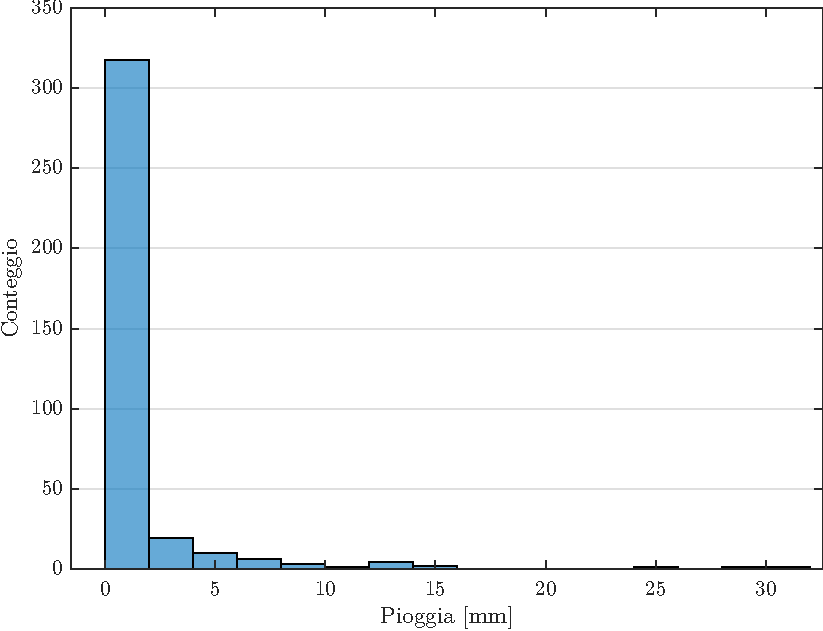
\includegraphics[height=133px]{Immagini/4. Caso di studio/Istogrammi/Istogramma, pioggia}\label{istogramma_pioggia}}\quad
	\subfigure[]{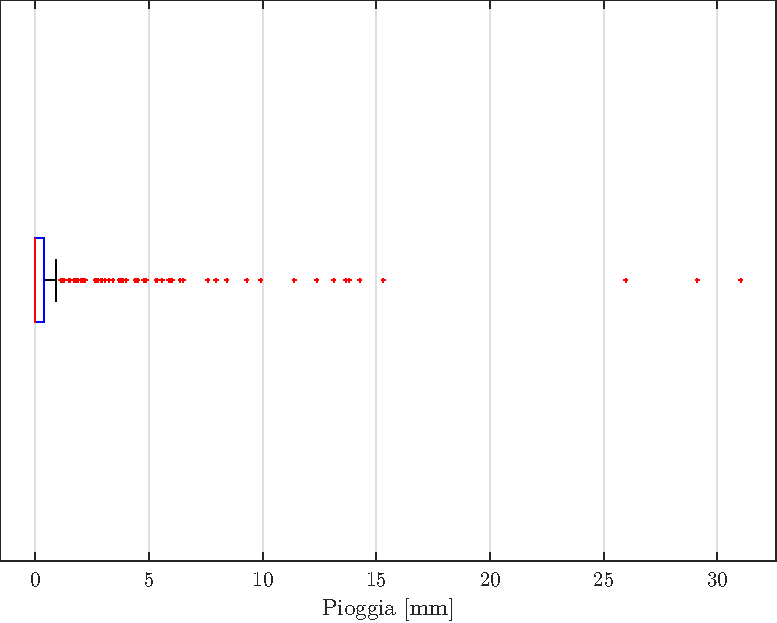
\includegraphics[height=133px]{Immagini/4. Caso di studio/Box-plot/Box-plot, pioggia}\label{boxplot_pioggia}}\quad
	\subfigure[]{\includegraphics[height=133px]{Immagini/4. Caso di studio/Istogrammi/Istogramma, visibilità}\label{istogramma_visibilità}}\quad
	\subfigure[]{\includegraphics[height=133px]{Immagini/4. Caso di studio/Box-plot/Box-plot, visibilità}\label{boxplot_visibilità}}
	\caption[Istogrammi e box-plot delle variabili meteorologiche, parte \num{1}]{istogrammi e box-plot delle varibili meteorologiche, parte \num{1}.}
	\label{istogrammi_boxplot_variabili_meteo_1}
\end{figure}

\begin{figure}[htpb]
	\centering
	\subfigure[]{\includegraphics[height=133px]{Immagini/4. Caso di studio/Istogrammi/Istogramma, velocità vento}\label{istogramma_vento}}\quad
	\subfigure[]{\includegraphics[height=133px]{Immagini/4. Caso di studio/Box-plot/Box-plot, velocità vento}\label{boxplot_vento}}\quad
	\subfigure[]{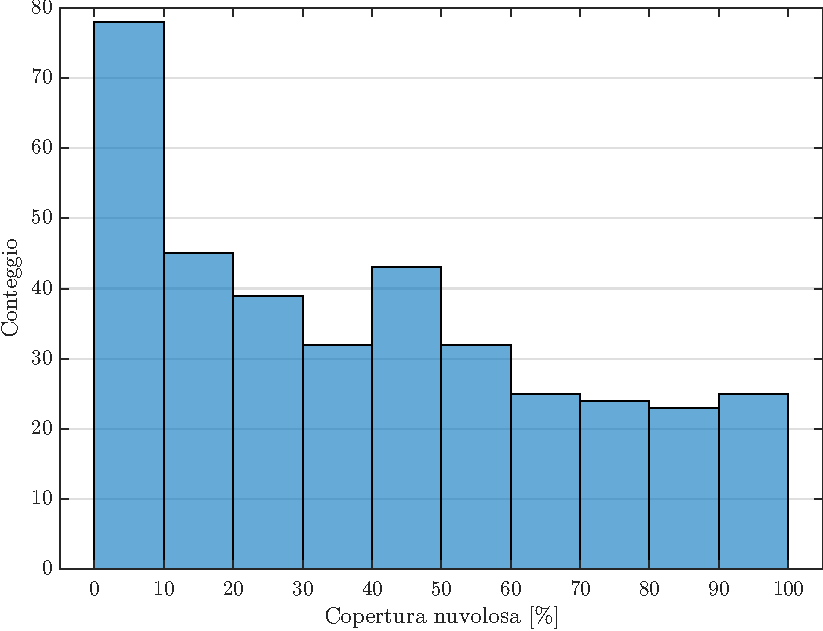
\includegraphics[height=133px]{Immagini/4. Caso di studio/Istogrammi/Istogramma, copertura nuvolosa}\label{istogramma_copertura}}\quad
	\subfigure[]{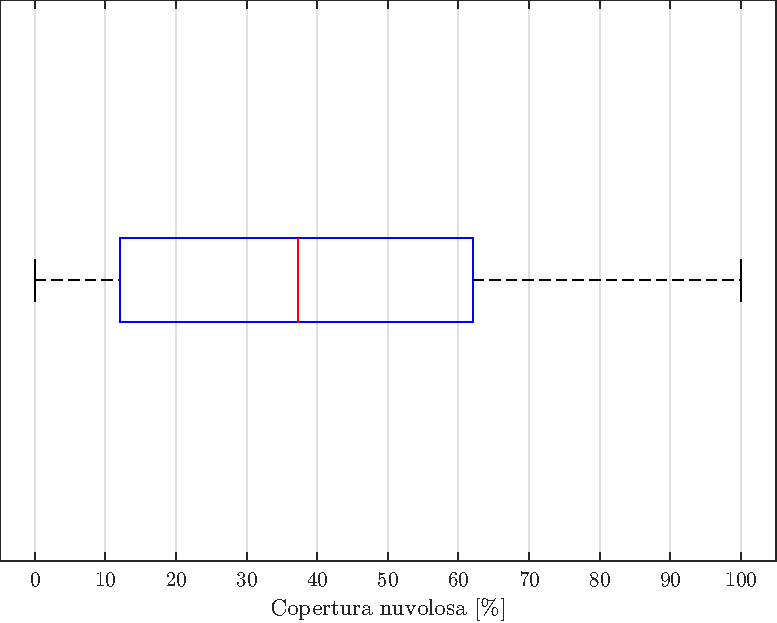
\includegraphics[height=133px]{Immagini/4. Caso di studio/Box-plot/Box-plot, copertura nuvolosa}\label{boxplot_copertura}}\quad
	\caption[Istogrammi e box-plot delle variabili meteorologiche, parte \num{2}]{istogrammi e box-plot delle varibili meteorologiche, parte \num{2}.}
	\label{istogrammi_boxplot_variabili_meteo_2}
\end{figure}

\begin{figure}[htpb]
	\centering
	\subfigure[]{\includegraphics[height=133px]{Immagini/4. Caso di studio/Serie storiche/Ritiri giornalieri e visibilità}\label{ritiri_vs_visibilita}}\quad
	\subfigure[]{\includegraphics[height=133px]{Immagini/4. Caso di studio/Serie storiche/Ritiri giornalieri e velocità vento}\label{ritiri_vs_vento}}\quad
	\caption[Confronto tra il numero medio di noleggi giornaliero, la visibilità orizzontale e la velocità del vento]{confronto tra il numero medio di noleggi giornaliero, la visibilità orizzontale (a) e la velocità del vento (b).}
	\label{ritiri_vs_variabili_meteo_2}
\end{figure}